\chapter{From Word Vectors to Agents}
\label{chapter:HowWeGotHere}
% EVOLVE-BLOCK-START

The agentic systems this course builds rest on large language models, and those models can seem to have arrived all at once.
They did not.
The capability that makes an agent possible (a single model that reads instructions, holds a conversation, writes code, and calls tools) is the accumulated payoff of a collection of significant advances, each of which removed a concrete limitation of the one before it.
This chapter traces that lineage at a high level, highlighting a few milestones.
The goal is not to teach any one method but to give the reader a timeline they can hold in their head: enough of the story to see that today's models are a consequence rather than an accident, and to talk with some fluency about how the field arrived here.

A single question runs through the whole progression, asked in progressively more powerful ways: how should a machine represent and manipulate language?
Each answer below made the next one reachable.
The dates are close together; the span from the first contributions outlined below to working agents is little more than a decade.
This is part of why the current moment feels sudden even though the path is legible in hindsight.

\section{Meaning as Geometry (2013--2014)}
\label{section:MeaningAsGeometry}

An imprtant step was to give words a form a machine could compute with.
A \emph{word embedding}\index{Word embedding} maps each word to a vector so that words with similar meanings land near one another, and the \emph{word2vec}\index{word2vec} models showed that such a space could be learned cheaply from raw text at scale (Mikolov et al., 2013).
A companion result added an efficient training objective and vectors for phrases, and displayed the now-famous regularity that simple vector arithmetic is meaningful in this space --- adding the vectors for \emph{Germany} and \emph{capital} lands near the vector for \emph{Berlin} (Mikolov et al., 2013).
Meaning had become geometry: a trained space in which distance encodes similarity.
This is the direct ancestor of the embeddings the course uses for retrieval (Chapter~\ref{chapter:Retrieval}, Definition~\ref{definition:Embedding}), one representational level down, words rather than passages.

Representing single words is not the same as handling a whole sentence.
The next step was to map an entire input sequence to an entire output sequence.
\emph{Sequence-to-sequence}\index{Sequence-to-sequence} learning used one recurrent network to compress an input sentence into a fixed-length vector and a second to decode an output sentence from it, trained end to end, and reached competitive machine translation with no hand-built linguistic machinery (Sutskever et al., 2014).
Its weakness was precisely that single fixed vector: forcing an entire sentence through one bottleneck lost information on long inputs.
Removing that bottleneck was the next breakthrough.

\section{The Transformer and the Age of Scale (2017--2018)}
\label{section:TransformerEra}

\emph{Attention}\index{Attention} came first as a patch to the bottleneck: additive attention let a recurrent decoder look back over all of the encoder's states rather than a single summary vector (Bahdanau et al., 2015), which relieved the pressure on long inputs but kept the sequential recurrence.
The \emph{Transformer}\index{Transformer} took the more radical step of discarding recurrence entirely and building the model out of attention alone (Vaswani et al., 2017).
It let every position in a sequence attend directly to every other, and made it practical to train much larger models on much more data because attention is parallel where recurrence is serial.
Every large language model the course uses is a Transformer.
Its attention mechanism is also why context has a cost: because attention normalizes its weights with a softmax over all positions, each added token dilutes the weight any single token can receive, so a finite attention budget is spread more thinly as the input grows; this effect is developed in Chapter~\ref{chapter:ContextEngineering}.

The Transformer was an architecture; the next move was a \emph{recipe} for using it.
Rather than train a fresh model for every task, one could \emph{pre-train}\index{Pre-training} a single Transformer on a large corpus of unlabeled text and then adapt it to specific tasks with comparatively little further training.
\emph{BERT}\index{BERT} did this with a bidirectional encoder trained to fill in masked words, producing \emph{contextual} representations --- a word's vector now depends on the sentence around it --- and set new results across many language tasks at once (Devlin et al., 2019).
Contextual embeddings from this family are what many modern retrieval actually runs on, the successor to the static word vectors of the previous section.
A parallel line pre-trained \emph{decoder} models for generation rather than understanding; that branch is the one that leads to the models an agent is built from.

\section{Scale, Prompting, and Grounding (2020)}
\label{section:ScaleAndGrounding}

Scaling the decoder branch produced a qualitative change, not merely a quantitative one.
\emph{GPT-3} was a 175-billion-parameter model that, with no task-specific training, could perform a new task from a plain-language instruction and a handful of examples placed in its context window: \emph{in-context}, or \emph{few-shot}, learning\index{In-context learning} (Brown et al., 2020).
This is the origin of prompting as the primary interface: the model is steered by the text it is given rather than by gradient updates, which is the premise the entire course operates on (Chapter~\ref{chapter:ContextEngineering}).
It is also where the honest limits come into view; few-shot performance is uneven, and training on web-scale text raises the leakage and contamination concerns the evaluation chapter takes seriously (Chapter~\ref{chapter:Evaluation}).

A frozen model's knowledge is fixed at training time: it cannot cite its sources, and it is hard to update.
\emph{Retrieval-augmented generation}\index{Retrieval-augmented generation} addressed this by pairing the model's parametric memory with a non-parametric one: retrieve relevant passages from an external corpus, then generate an answer conditioned on them (Lewis et al., 2020).
This made knowledge updatable and attributable, and it is a basis of the grounding developed in Chapter~\ref{chapter:Retrieval}.

\section{From Models to Agents (2022 onward)}
\label{section:FromModelsToAgents}

A capable, promptable model is still not an agent.
Three further developments closed that gap.
\emph{Instruction tuning} with human feedback aligned models to follow instructions helpfully rather than merely continue plausible text, making their behavior reliable enough to direct (Ouyang et al., 2022).
\emph{Chain-of-thought} prompting showed that eliciting intermediate reasoning before a final answer improves performance on multi-step problems (Wei et al., 2022).
And giving the model \emph{tools} --- letting it act, observe the result, and act again --- turned a text generator into a system that operates in the world, formalized as the reason-and-act loop the course builds in Chapter~\ref{chapter:AgentLoop} (Yao et al., 2023).
At that point the model is no longer only answering; it is perceiving, reasoning, and acting.

The chain did not stop at tool use.
The most recent step folds reasoning back inside the model: \emph{reasoning models}\index{Reasoning model} are trained to carry out extended chains of thought internally before they answer, rather than being prompted to reason step by step, and models are increasingly \emph{multimodal}, taking images and other data alongside text.
The practical consequences, including a latent reasoning trace that cannot be read as an audit log and a thinking budget in place of a prompt scaffold, are treated in Chapter~\ref{chapter:AgentLoop}.
The progression this chapter traces is therefore still under way, but its shape is unchanged: each step extends what the system can reliably do on its own.

\section{The Progression Was Not Random}
\label{section:NotRandom}

Read as a list, the milestones above are a handful of loosely related papers.
Read as a chain, each one removed a specific limitation of the last.
Word vectors gave meaning a computable form but handled only isolated words; sequence-to-sequence mapped whole sentences but squeezed them through one vector; the Transformer removed that bottleneck and made scale practical; pre-training made a single model's knowledge transferable across tasks; scale made that model steerable by plain text; retrieval grounded it in external, updatable knowledge; and instruction tuning and tool use let it act.
Table~\ref{table:AgenticTimeline} lists the sequence; Figure~\ref{figure:AgenticChain} draws it as the dependency chain the prose describes, each arrow labelled with the limitation the next step removed.

\begin{figure}[t]
\centering
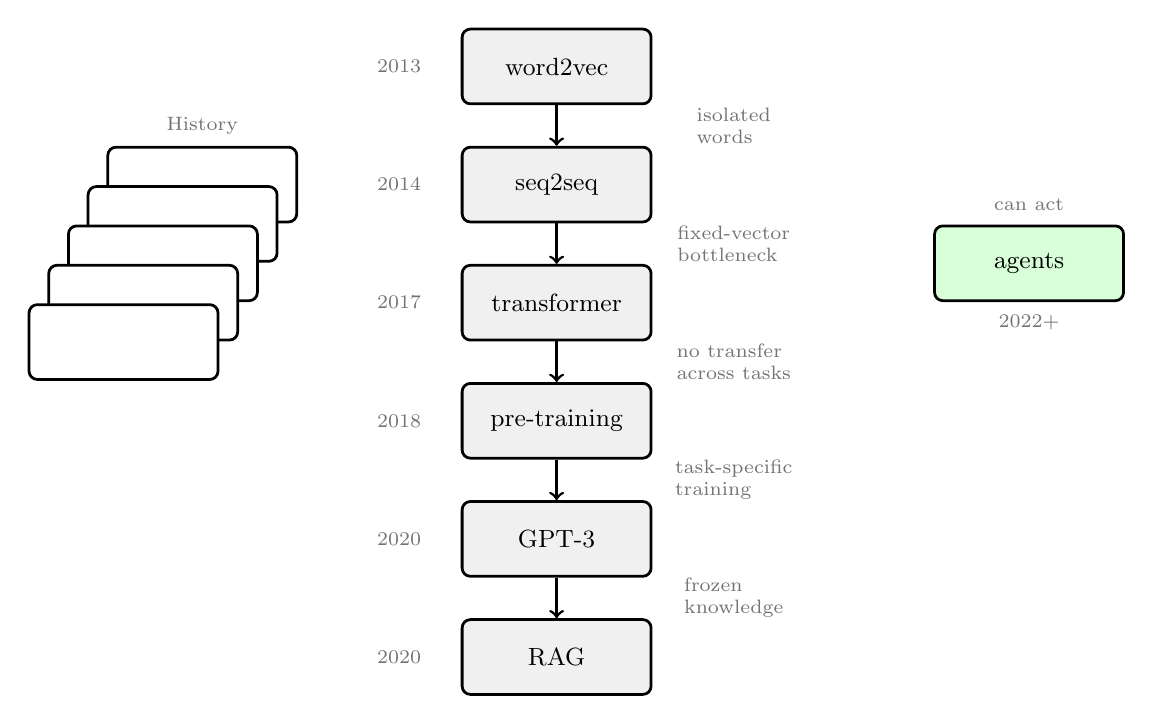
\begin{tikzpicture}[
  font=\small, line width=1pt,
    box/.style={draw, rounded corners=3pt, minimum width=2.4cm, minimum height=0.95cm,
                align=center, font=\small, fill=gray!12},
    hbox/.style={draw, rounded corners=3pt, minimum width=2.4cm, minimum height=0.95cm,
                align=center, font=\small, fill=white},
    lim/.style={font=\scriptsize, text=black!55, align=left},
    yr/.style={font=\scriptsize, text=black!55},
]
\node[hbox] (h1) at (1.5,6) {};
\node[hbox] (h2) at (1.25,5.5) {};
\node[hbox] (h3) at (1,5) {};
\node[hbox] (h4) at (0.75,4.5) {};
\node[hbox] (h5) at (0.5,4) {};
\node[lim] at (1.5,6.75) {History};
\node[box] (n1) at (6,7.5) {word2vec};
\node[box] (n2) at (6,6) {seq2seq};
\node[box] (n3) at (6,4.5) {transformer};
\node[box] (n4) at (6,3) {pre-training};
\node[box] (n5) at (6,1.5) {GPT-3};
\node[box] (n6) at (6,0) {RAG};
\draw[->] (n1) -- (n2);
\draw[->] (n2) -- (n3);
\draw[->] (n3) -- (n4);
\draw[->] (n4) -- (n5);
\draw[->] (n5) -- (n6);
\node[lim] at (8.25,6.75) {isolated\\words};
\node[lim] at (8.25,5.25) {fixed-vector\\bottleneck};
\node[lim] at (8.25,3.75) {no transfer\\across tasks};
\node[lim] at (8.25,2.25) {task-specific\\training};
\node[lim] at (8.25,0.75) {frozen\\knowledge};
\node[yr] at (4,7.5) {2013};
\node[yr] at (4,6) {2014};
\node[yr] at (4,4.5) {2017};
\node[yr] at (4,3) {2018};
\node[yr] at (4,1.5) {2020};
\node[yr] at (4,0) {2020};
\node[box, fill=green!15] (n7) at (12,5) {agents};
\node[yr] at (12,4.25) {2022+};
\node[lim] at (12,5.75) {can act};
\end{tikzpicture}
\caption{The lineage as a causal chain.
Each box is a milestone, with its year below; each arrow is labelled with the limitation of the step on its left that the step on its right removed.
The point is not the list of names but the dependency between them: representing isolated words made mapping whole sequences the next problem, whose fixed-vector bottleneck made attention the next, and so on until a model that can act --- an agent.}
\label{figure:AgenticChain}
\end{figure}

\begin{table}[t]
\centering
\caption{A high-level timeline of the milestones behind agentic language models.
Each step removed a concrete limitation of the previous one; the course develops the ideas in the right-hand column in the chapters they anchor.
Years mark when each result first appeared as a preprint; the publication venues given in the Further Reading sometimes lag by a year, as with BERT (2018 preprint, NAACL~2019).}
\label{table:AgenticTimeline}
\begin{tabular}{@{}l l p{8.3cm}@{}}
\toprule
Year & Breakthrough & What it unlocked \\
\midrule
2013  & Word embeddings                   & meaning as a learned vector geometry \\
2014  & Sequence-to-sequence              & end-to-end mapping of whole sequences \\
2017  & The Transformer                   & attention replaces recurrence; scale becomes practical \\
2018  & Pre-training                      & transferable, contextual representations \\
2020  & Scale and few-shot                & steering a frozen model by text alone \\
2020  & Retrieval-augmented generation    & grounding in external, updatable knowledge \\
2022--23 & Chain-of-thought               & following instructions and acting --- agents \\
2024--26 & Reasoning \& multimodality     & trained latent reasoning; the chain continues \\
\bottomrule
\end{tabular}
\end{table}

None of these steps was guaranteed in advance, and their nearness in time is why the field's current state is genuinely recent.
But the sequence is not arbitrary: today's agents are where this particular chain of problems and solutions has led, and the same pressure that drove it --- extend what the system can reliably do --- is what drives the rest of these notes.
With the timeline in place, the next chapter turns from how we got here to what an agent is, and why general-purpose tool-using models can accelerate research and discovery.

\section*{Further Reading}

\begin{small}
\begin{enumerate}
\item Mikolov, T., Chen, K., Corrado, G., and Dean, J., ``Efficient Estimation of Word Representations in Vector Space,'' \emph{ICLR Workshop}, 2013 — the word2vec architectures (CBOW and Skip-gram).
\item Mikolov, T., Sutskever, I., Chen, K., Corrado, G., and Dean, J., ``Distributed Representations of Words and Phrases and their Compositionality,'' \emph{NeurIPS}, 2013 — negative sampling, phrase vectors, and additive compositionality.
\item Sutskever, I., Vinyals, O., and Le, Q. V., ``Sequence to Sequence Learning with Neural Networks,'' \emph{NeurIPS}, 2014 — the recurrent encoder--decoder.
\item Bahdanau, D., Cho, K., and Bengio, Y., ``Neural Machine Translation by Jointly Learning to Align and Translate,'' \emph{ICLR}, 2015 — additive attention within a recurrent model, the first relief of the fixed-vector bottleneck.
\item Vaswani, A., et al., ``Attention Is All You Need,'' \emph{NeurIPS}, 2017 — the Transformer; attention alone, recurrence removed; the architecture underlying every model the course uses.
\item Devlin, J., Chang, M.-W., Lee, K., and Toutanova, K., ``BERT: Pre-training of Deep Bidirectional Transformers for Language Understanding,'' \emph{NAACL}, 2019 — pretraining and contextual representations.
\item Brown, T. B., et al., ``Language Models are Few-Shot Learners,'' \emph{NeurIPS}, 2020 — GPT-3 and in-context learning.
\item Lewis, P., et al., ``Retrieval-Augmented Generation for Knowledge-Intensive NLP Tasks,'' \emph{NeurIPS}, 2020 — parametric plus non-parametric memory.
\item Ouyang, L., et al., ``Training Language Models to Follow Instructions with Human Feedback,'' \emph{NeurIPS}, 2022 — instruction tuning with human feedback.
\item Wei, J., et al., ``Chain-of-Thought Prompting Elicits Reasoning in Large Language Models,'' \emph{NeurIPS}, 2022 — intermediate reasoning before an answer.
\item Yao, S., et al., ``ReAct: Synergizing Reasoning and Acting in Language Models,'' \emph{ICLR}, 2023 — interleaving reasoning with tool use.
\end{enumerate}
\end{small}
% EVOLVE-BLOCK-END
